\documentclass[12pt]{scrartcl}
\title{Assignment 6\\ Paper Prototyping for\\ Evaluation and Reporting}
\author{\textbf{Flow Overstack Team}\\ Cesana Filippo\\ Folli Gary\\ Hartmann Kathrin\\ Rodolfo Masera Tommaso\\ Stucchi Jacopo\\ Taillefert Stefano}
\date{}
\setlength{\parindent}{0pt}

\usepackage{graphicx}
\usepackage{subfig}
\usepackage{float}
\usepackage[margin = 2.5cm]{geometry}


\begin{document}

\maketitle

\tableofcontents

\newpage

\section{Introduction}

	% Start your report by describing briefly your app and refer back to your concept statement. Should this statement be outdated (i.e., not fit the design that was developed by your group), provide an updated version.
	
	Our app - V.I.P. - aims to merge education and social media. By taking a picture of a person, the app associates the face of such a person with a key personality of the past or of the present. After having discovered a new historical profile, the user can share her discovery with her friends on the feed. Of course, this process works also the other way round: by reading the feed, the user can collect new information about a certain VIP who has been unveiled by her friends.\\
	
	The education part goes hand in hand with our app thought-provoking name. We indeed tried to challenge that nowadays ephemeral conception of VIP which has conquered social media - such as Instagram, for example - where fame and merit are based on the appearance and therefore lie on a superficial ground. On the contrary, our VIPs are people who have changed society, politics, arts, language, science, philosophy and so on, such as Giotto, Alan Turing, Jean Baudrillard and so on.\\
	
	Since learning about historical people may be perceived as boring due to the connections which school has established with this type of study, we have tried to make our app as social as we could. Not only we have looked closely at the GUI of successful social media - such as the aforementioned Instagram - to build a solid and captivating interface, but we have also conceived the camera as a playful tool which could keep our young users as entertained as possible, thus ultimately changing the way through which they may have experienced this kind of learning process so far.\\
	
	But of course, our best proposes needed a feedback from our persona, that is from the ideal user to whom we are dedicating this app - naturally, despite having a particular user in our mind, our app still extends its range to everyone who is able to read and willing to learn a little of general culture. Therefore, various types of feedback paper have been elaborated during the various stages of this group project. Similarly, the shown material related to the app has changed along the way. For this last phase, we were able to present to our users a fully functional prototype of our app, developed with Adobe XD. In terms of feedback, we tried a new technique which, among the other things, could have eliminated some of the ambiguity collected through the users feedback during the past stages of the project. This feedback strategy, as well as our prototype, and key tasks, usability problems and much more will be further explained and explored in the next sections. 

	\newpage	
	
\section{Paper Prototyping}

	% Describe very briefly the paper prototyping process you used.
	
	// TODO - Jacopo
	
	
\section{Key Tasks}

	% Show here the list of key tasks you used to drive the inspection process. Mention whether you defined different tasks for children and why.
	
	As described in our last report, the main purpose of the key tasks that we devised is to determine 
	whether the wireframe and interface we designed is clear enough for our end users:
	
	\begin{itemize}
	\item  \textbf{Creating an Account and Logging In} Firstly, entering the application itself should
	not pose to the user any difficulty, so we want to test if it is as intuitive as possible.
	
	\item \textbf{Taking a Picture and Discovering a Famous Person} As this is the application's main
	feature and selling point, it is a must to test that it works correctly.
	
	\item \textbf{Adding the Discovered Person to the Gallery} This is to see if the user
	understands the main concept of the app, which is to unlock and collect the famous people
	they came across.
	
	\item \textbf{Navigating the Gallery to see other Character Descriptions} This aligns with the
	collecting and unlocking point from above. Moreover, it helps us know whether our interface is
	easy to traverse.
	
	\item \textbf{Viewing a Friend's Profile} This is meant to test the social aspect of our application
	such that it is clear to the user how the friend requests and friends' profiles work.
	
	\item \textbf{Finding and Using the Settings Menu} As a last task we want the user to open the
	settings menu. This is, again, to test whether the interface is clear. Since it is not the main point
	of the application it does not mean that the user should feel lost when looking for the settings.
	\end{itemize}
	
	\paragraph{\large Field-Testing Results}
	
	Overall, the test users performed really well. They followed through with every task smoothly and
	didn't meet any particular difficulties in navigating the wireframe. What we gathered from this
	testing is that the interface is conceptually sound and shouldn't make the user question the
	functionalities of the application. The only negative we found is that the settings menu was harder
	to find as it is only viewable from the user's own profile. This can easily be dealt with in a more
	polished prototype as we can look into making it more visible.
	
	\newpage

\section{Usability Problems}

	% Show here the list of usability problems you compiled in the inspection process, and point out similarities and differences when engaging children vs young adults.
	
	Generally speaking, the testing with both our peers and the children went very smoothly, as we were never left with a completely lost user or terrible complaints. Everyone had a vague idea of what the app should do and the children even remembered us from the video we shoved them back in April.\\
	
	The interaction we had with the users were very similar between children and adults, even some complaints or suggestions were the same; everyone navigated throughout the app and achieved the tasks quite easily or simply needed one small hint to reach their goal. We think (and our users say, see the "Statistics" section) that the app is intuitive and clear to use, so this could be one reason for the smoothness of the testing. We also had very enthusiast and collaborative users, both at USI and at Istituito Elvetico, which was very helpful for us and simplified the whole process.\\
	
	There were some minor issues that, in our opinion, can easily be addressed by redesigning some parts of the UI or by adding tips or small explanations and tutorials.\\
	One example is the rarity stars (see Figure \ref{stars} below), which many users believed to be clickable when they were merely an indication of the rarity of the VIP; in that case, a better design for the icons (filled instead of just an outline) could be a simple yet effective solution.\\
	
	\begin{figure}[H]
		\centering
		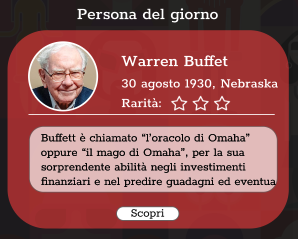
\includegraphics{../images/GA6_Stars.png}
		\caption{The rarity stars, mistaken to be clickable}
		\label{stars}
	\end{figure}
	
	\newpage
	
	
\section{Statistics}

	% Extract data from the pictures of the keywords feedback and summarize it

	After the development of the prototype using Adobe XD, a very complete program for designing and prototyping mobile applications and websites, we now collected a variety of results. Our app prototype was not only very realistic, it was also possible to emulate its functioning using a program. Thus, we were allowing our testers (users) to concretely judge the application content and its functionalities in terms of user interface and user experience. \\

	To this end, two testing sessions were conducted, one with our peers, which do not represent concretely the target users, and a more one representative with the children. The feedbacks were collected using a keyword mapping technique where the users had to choose between 1 and 12 words out of 36, which represented our application best from their point of view, placing them on a paper and every time justifying why they chose those specific word.\\

	Again, the feedbacks collected were qualitative and we decided, firstly, to make an enumeration of the different keywords used and for every one of them, choosing if the word is positive or negative. Secondly, we will go through the feedback to take out the positive and negative aspects of our application with respect to the words list. Finally, with these data, we will analyze how we can improve our applications and which sides specifically by taking in account the feedback and the suggestions.\\

	Below is the compilation of all words used during the 10 peers feedbacks on the left column and the 3 children’s feedbacks on the right column. It would have been very useful to have more children’s feedbacks (at least five, according to Nielson) as we can really see a sort of tendency in the word used when compiling a certain amount of them. Both columns are sorted by the number of times a word appeared in the different feedbacks. The white lines represent the neutral or positive words, whereas the red lines are the clearly negative words. As we can see, the records are rather very positive. Indeed, on both sides (peers and children), our application is described as:\\
	
		- Interesting and innovative concept;\\
		
		- Organized, simple, clear, intuitive and easy in the general usability;\\
		
		- Inviting, smooth, persuasive, fresh, concise and clean in the design and interface;\\
		
		- Useful, helpful and appropriate in a general manner for the user;\\
	
		- Dull by two feedbacks;\\
		
		- Incomprehensible, confusing, dated, overwhelming, unattractive and unpredictable by one feedback each respectively.\\

	The negative aspects represent a rather minority with 9 negative words against 145 rather positive (or neutral), that is to say a 94\% of positive denominators against a 6\% of negative ones.
	
	\newpage

	\begin{figure}[H]
		\centering
		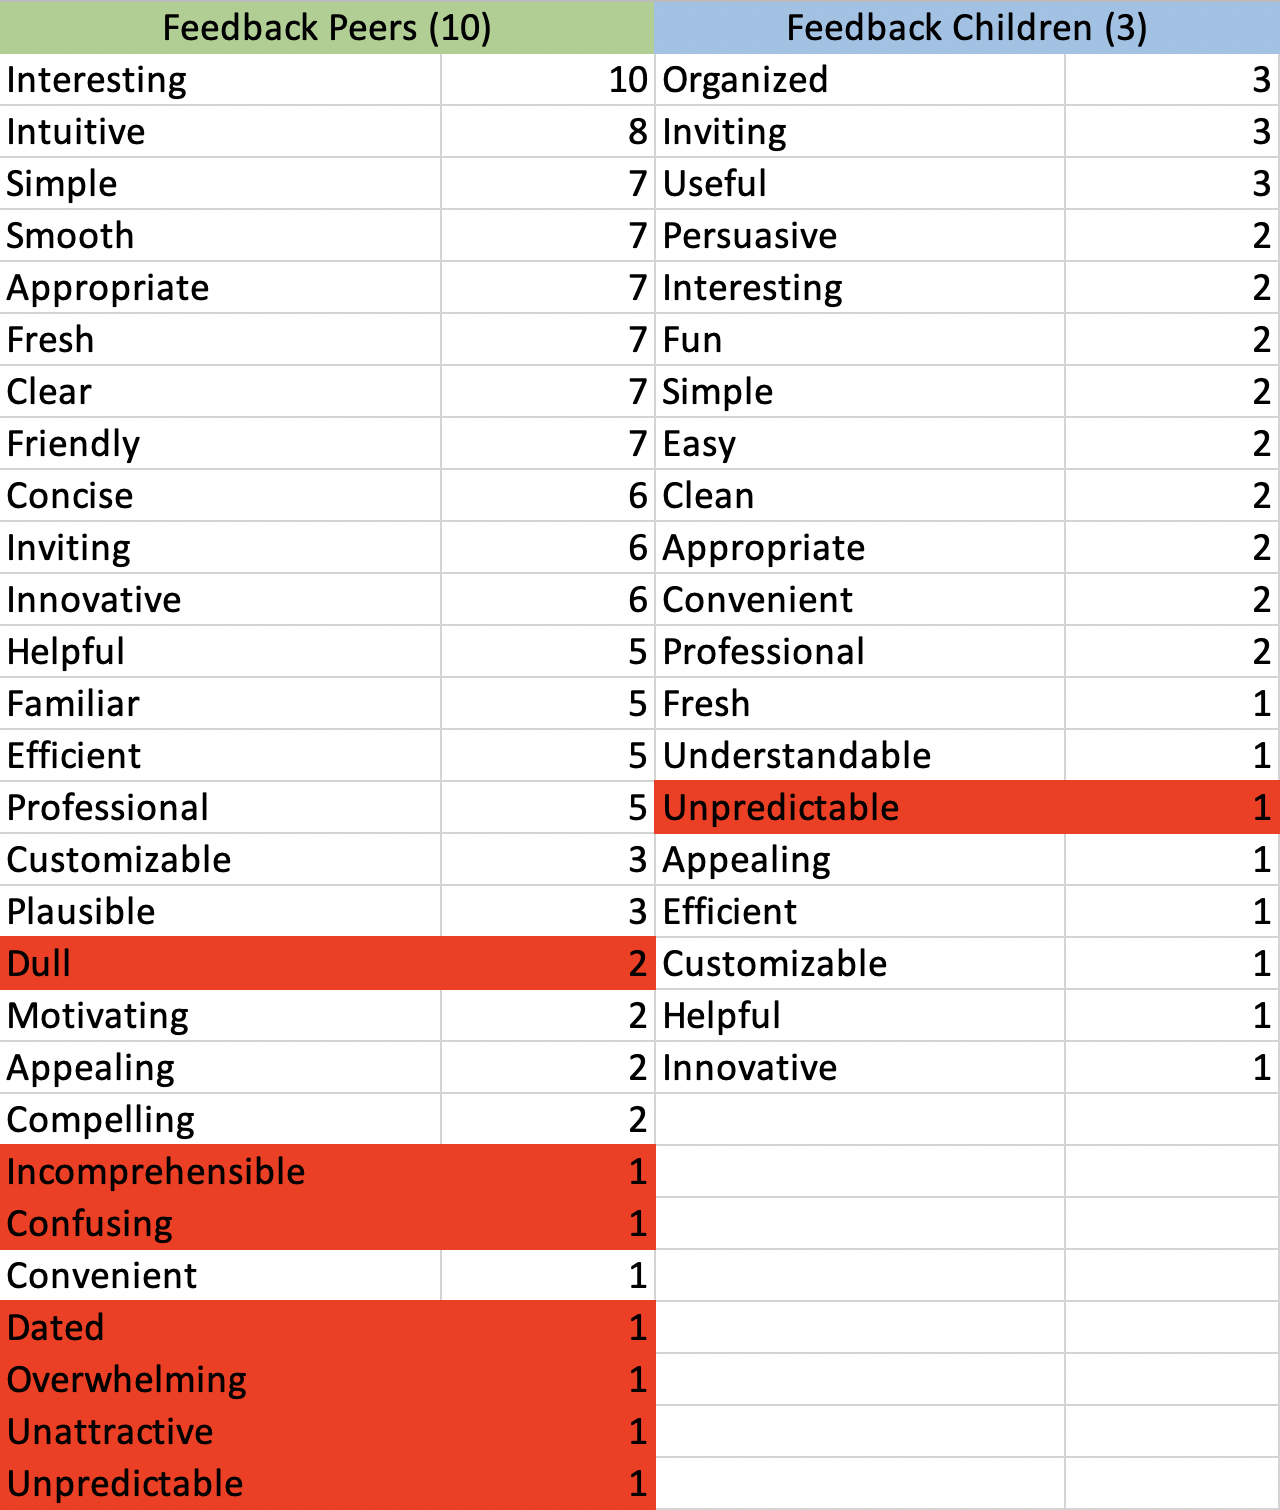
\includegraphics[width=\textwidth]{../images/gary_GA6_image_words_analysis.png}
		\caption{The keywords distribution}
		\label{words}
	\end{figure}
	
	\newpage

	Now we come to the associated feedbacks. Globally, they have been very positive:\\

		- The graphical interface (the design in general) was appreciated very much. It makes the application appealing and pushes people to try it and play with it;\\

		- The user experience and the functionalities were also among the positive aspects. The navigation was described as clear, clean and intuitive. Apart from some functionalities like finding a friend which were more difficult to find and the settings for which the access is described as unpredictable, the other functionalities were very user-friendly;\\

		- A lot of feedbacks pointed out the usefulness of the applications and the educative aspect, which can be revealed as very helpful for children. Quite surprisingly, even though our idea seemed unclear at the beginning, it is now accepted as an original and very interesting concept and above all, potentially very useful for the users;\\

		- The negative feedbacks, particularly the fact that the application is described as dull, overwhelming and unattractive, come from the educative aspect, which somehow killed the game aspect and thus led to a potentially boring application. Concerning the dated aspect, it was pointed out due to the fact that nowadays the internet offers hundreds of other possibilities for learning: MOOC, YouTube documentaries, ... which can be more interesting than reading texts on an app.\\
		\newline

	Finally, the interesting suggestions given by the users were the following:\\

		- Refactoring the way information is presented about the famous personages. The long texts are described as boring and not inviting, we should rather put some key facts. In the same idea, a user suggested the implementation of quizzes about the personages to reinforce game and educative aspects at the same time. Moreover, another user suggested the implementation of videos (small documentaries) instead of texts for each famous personage;\\

		- In terms of usability, a tutorial at the beginning of the app would be really useful. A minor suggestion was about adding the possibility to order our personages by rarity, name, dates, ...\\

		- Last but not least, a commentary, which was already made during the questionnaire in the last paper prototypes, concerns the facial recognition. It seems that users tend to find it unpredictable as they don’t really understand how it could compare their faces with the one of actual famous personages. Even if this functionality is part of the core of the app, it is true that maybe some refactoring and improvement should be made on this part as it seems still unclear for the users how the facial recognition really works.
		
		\newpage

	
\section{Conclusion}

	% A brief statement reflecting on how the process worked (or didn't) for your team and any important lessons learned.
	
	Taking all this into consideration, it can be said that the development process of our application was very successful.\\

	Going through the many steps of the development process, we got an idea of how complex app development from the point of view of Human-Computer Interaction is and how many thoughts are behind a successful app idea. From the first concept statement over the work-activity-affinity diagram, the wireframes and storyboards, the prototype development and last but not least the usability testing, our knowledge of UX Design got deeper and deeper and our app idea step to step more precise.\\
	
	An important lesson learned was recognizing the usefulness of having usability tests: Although we were putting very much efforts in designing a user-optimized application, we overlooked some obvious faults in the design. We learned that you should always test your application before declaring it as complete. Already a few tests are enough to detect the main faults. We will remember this for our future developer career.\\
	
	Another important point is the work with kids as user group. We were impressed how friendly, cute but also brutally honest they were when writing the feedbacks. Moreover, it was awesome how well they recognized our app idea again just from a short one-minute video, when we were performing the usability test.\\
	
	Finally, our skills in working and organizing ourselves in a group improved a lot. We learned how to divide tasks properly, and how to develop a team spirit. Furthermore, we faced how to manage problems with different languages, regarding talking to our user group, the kids, and then implementing their feedback in our application.
	
	
\end{document}